% die Standard-Dokumentenklasse
\documentclass[11pt,a4paper]{article} %% 1.Ebene = chapter, headings

% input encoding, font encoding, outline font
\usepackage[utf8]{inputenc} 
\usepackage[T1]{fontenc} 
\usepackage{lmodern}
\usepackage{tcolorbox}
% Sprache
\usepackage[german]{babel}

% Absatzformatierung
\setlength{\parindent}{0pt}
\setlength{\parskip}{1ex plus 0.5ex minus 0.5ex}

% erweiterte mathematische Symbole
\usepackage{amsmath} 

% für Abbildungen
\usepackage{graphicx} 

% für Tabellen
\usepackage{booktabs}

% für Hyperlinks
\usepackage[colorlinks]{hyperref}
\graphicspath{}

%%%%%%%%%%%%%%%%%%%%%%%%%%%%%%%%%%%%%%%%%
\begin{document}
	
	
	{
		\centering 
		\large 
		Physiklabor für Anfänger*innen \\
		Ferienpraktikum im Sommersemester 2018 \\[4mm]
		\textbf{\LARGE 
			Versuch 38: Spezifische Wärmekapazität von Wasser
		} \\[3mm]
		(durchgeführt am 10.09.2018 bei Nico Strauß) \\
		Ye Joon Kim, Marouan Zouari\\
		\today \\[10mm]
	}
\section{Einleitung}
Die Erhaltung der Energie impliziert, dass die Energie in andere Formen umgewandelt werden können. Insbesondere können mechanische und elektrische Energie sich in thermische Energie umwandeln. Mit dieser Eigenschaft lässt sich die Wärmekapazität von Wasser bestimmt werden. 



\section{Ziel des Versuchs}
Das Ziel dieses Versuchs ist es, die spezifische Wärmekapazität von Wasser auf mechanische und elektrische Weise zu bestimmen.  
\section{Aufbau}

\begin{figure}
	\centering
	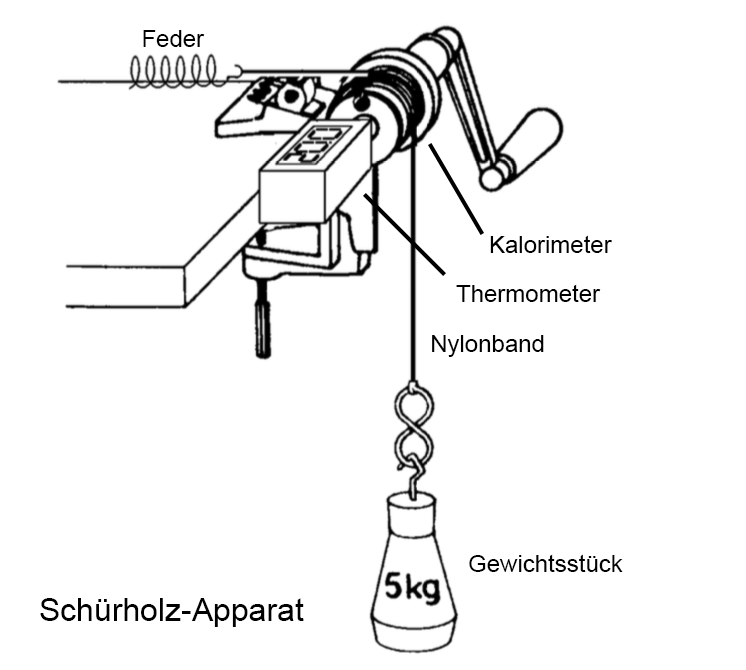
\includegraphics[scale=0.5]{fig1}
	\caption{Aufbau zum 1. Versuchsteil. ("Versuchsanleitungen zum Physiklabor")}
	
	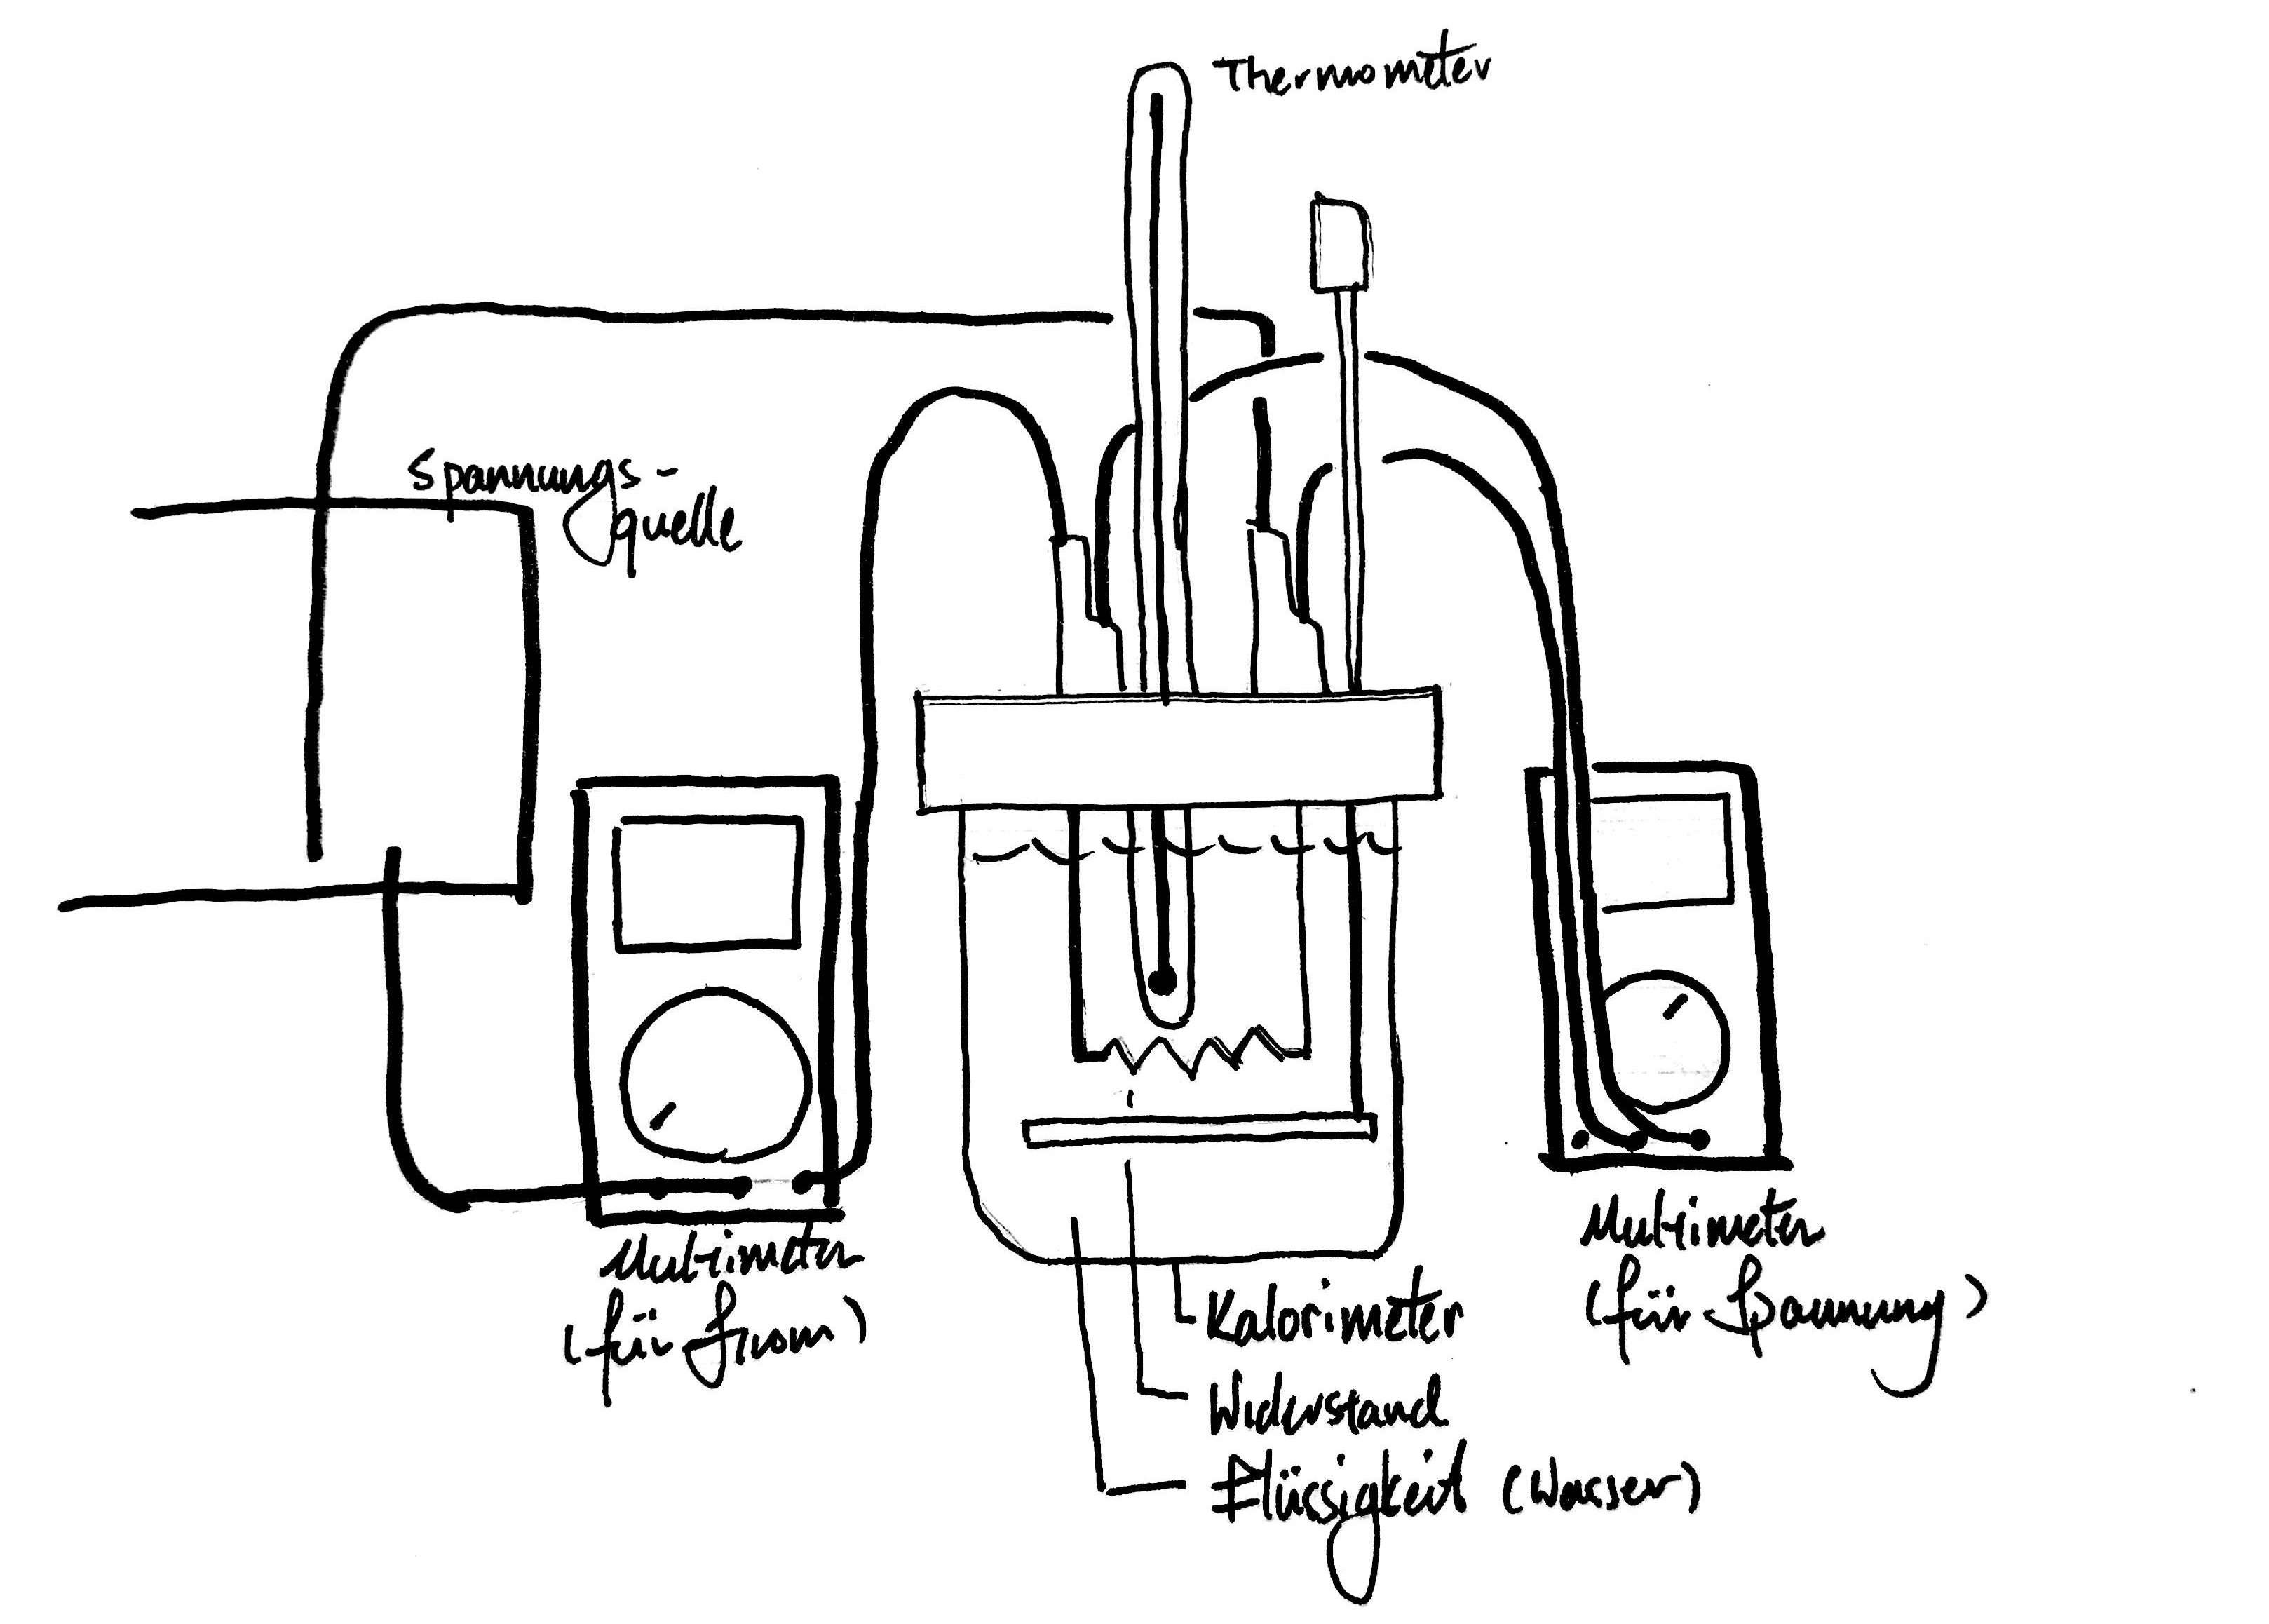
\includegraphics[scale=0.10]{fig2}
	\caption{Aufbau zum 2. Versuchsteil}
\end{figure}
\newpage

\section{Auswertung und Fehlerrechnung}
Rohe Daten sind in dem Anhang zu finden. 

\subsection{1. Versuchsteil:Mechanische Bestimmung der Wärmekapazität.}

Für die Bestimmung der Wärmekapazität wird die folgende Formel benutzt:
\begin{equation}
(\Gamma_{\textrm{Kal}}+\Gamma_{\textrm{T}}+m_\textrm{W}c_\textrm{W})\Delta T = mgn\pi d
\end{equation}
wobei:
\begin{itemize}
	\item $\Gamma_{\textrm{Kal}}$ Die Wärmekapazität des leeren Kalorimeters
	\item $\Gamma_{\textrm{T}}$ Die Wärmekapazität der Thermoelemententhalterung und des Nylonbands
	\item $m_\textrm{W}$ Die Masse des Wassers
	\item $c_\textrm{W}$ Die spezifische Wärmekapazität des Wassers
	\item $\Delta T$ die Temperaturunterschied
	\item $m$ die Masse des Massestücks
	\item $g$ die Fallbeschleunigung
	\item $n$ die Anzahl Drehungen
	\item $d$ der Durchmesser des Kalorimeters sind
\end{itemize}

Die Formel kann umgeformt werden, um einen Ausdruck für $c_\textrm{W}$ zu liefern:

\begin{equation}
c_\textrm{W} = \frac{\frac{mgn\pi d}{\Delta T} - \Gamma_{\textrm{Kal}} - \Gamma_{\textrm{T}}}{m_\textrm{W}}
\end{equation}



Es wurden vier Messungen durchgeführt. Die von den Einzelmessungen gewonnenen Werte für die spezifische Wärmekapazität und deren Unsicherheiten sind:


\begin{table}[h]
	\centering
	\begin{tabular*}{0.99\textwidth}{@{\extracolsep{\fill}}cccccc}
		\toprule
		Messreihe & $c_\textrm{W}$ & $\Delta c_\textrm{W})$  \\
		& J/kg K & J/kg K   \\
		1 & 5442 & 2000 \\
		2 & 5800 & 1100 \\
		3 & 6200 & 1300 \\
		4 & 6200 & 1300 \\
		\bottomrule
	\end{tabular*}
	\caption{Eine Tabellenunterschrift.}
	\label{tabelle}
\end{table}

\subsubsection{Beispielrechnungen (Mit ersten Datenpunkten)}
\hrule
\begin{tcolorbox}[colback=white]
Einfaches Einsetzen der Werte in Gleichung (2) liefert die jeweilige spezifische Wärmekapazitäten. 
$$c_\textrm{W} = \frac{\frac{mgn\pi d}{\Delta T} - \Gamma_{\textrm{Kal}} - \Gamma_{\textrm{T}}}{m_\textrm{W}}$$

$$ =\frac{ \frac{ 5 \textrm{kg} \cdot 9,8 \textrm{m/s}^2 \cdot 50 \cdot \pi \cdot 0,0472 \textrm{m}}{0,9^\circ C} - (380 \textrm{J/kg K} \cdot 0,098 \textrm{kg}) - 5 \textrm{J/K}}{0,066\textrm{kg}}$$
$$ = 5442,98 \textrm{J/kg K} $$
Und für die Fehlerrechnungen werden die Gauß'sche Fehlerfortpflanzung benutzt. Mit:
$$f(n,d,\Delta T,m_\textrm{W}) = \frac{\frac{mgn\pi d}{\Delta T} - \Gamma_{\textrm{Kal}} - \Gamma_{\textrm{T}}}{m_\textrm{W}}$$
sind:
$$ \frac{ \partial f}{\partial n} = \frac{mg\pi d}{\Delta T m_{\textrm{W}}} $$ 
$$ \frac{ \partial f}{\partial d}  = \frac{mgn\pi}{\Delta Tm_{\textrm{W}}}$$
$$ \frac{\partial f}{\partial \Delta T} = -\frac{(mgn\pi d)}{m_\textrm{W}} \frac{1}{\Delta T ^2}$$
$$ \frac{\partial f}{\partial m_{\textrm{W}}} = -(\frac{mgn\pi d}{\Delta T} - \Gamma_{\textrm{Kal}} - \Gamma_{\textrm{T}})
 \frac{1}{m_\textrm{W}^2}$$

$$\Delta c_\textrm{W} = \sqrt{ 
	(\frac{ \partial f}{\partial n} \Delta n)^2
	+(\frac{ \partial f}{\partial d} \Delta d)^2
	+(\frac{\partial f}{\partial \Delta T} \Delta (\Delta T))^2
	+ (\frac{\partial f}{\partial m_{\textrm{W}}} \Delta m_{\textrm{W}})^2 }
$$
$$ = 2026,25 \textrm{ J/kg K} $$

\end{tcolorbox}

Der Mittelwert der Werte und seine Standardunsicherheit lauten:
$$(5900 \pm 400) \textrm{ J/kg K}$$

Die Standardunsicherheit wurde mit der Formel:
\begin{equation}
s_x = \sqrt{\frac{\sum_{i=1}^{n}(x_i-\bar{x})^2}{n-1}} 
\end{equation}

berechnet. 

\section{2. Versuchsteil}

Für die elektrische Methode muss die von dem Widerstand abgestrahlten Energie bestimmt werden. Das kann mit der folgenden Relation bestimmt werden:
$$ W = Q = UI\Delta T $$

\begin{table}[h]
	\centering
	\begin{tabular*}{0.99\textwidth}{@{\extracolsep{\fill}}cccccc}
		\toprule
		Messreihe & $\Delta t$ & $\Delta(\Delta t)$ & $Q$ & $\Delta Q$  \\
		& s & s & J  & J  \\
		1 & 150 & 2 & 8900 & 100 \\
		2 & 210 & 2 & 10200 & 100 \\
		3 & 360 & 2 & 17600 & 100 \\
		\bottomrule
	\end{tabular*}
	\caption{Eine Tabellenunterschrift.}
	\label{tabelle}
\end{table}

Für die Berechnung der Unsicherheiten von $Q$ wurde die vereinfachte Formel für Produkte und Quotienten benutzt, und für die von $\Delta t$ die Formel für Summe. 

Zur Bestimmung der $T_\textrm{End}$, die maximale Temperatur ohne Verlust und Verzögerungseffekte, wurde das Extrapolationsverfahren benutzt. Nur die Datenpunkten von der Abfallphase wurden genommen und in einem Excel Dokument, das die lineare Regression automatisch berechnet,  eingesetzt. Die berechneten Werte für $a$ und $b$, Achsenabschnitt und Steigung, sind: 



\begin{table}[h]
	\centering
	\begin{tabular*}{0.99\textwidth}{@{\extracolsep{\fill}}cccccc}
		\toprule
		Messreihe & $a$ & $u_a$ & $b$ & $u_b$\\
		& $^\circ$ C & $^\circ$ C & $^\circ$ C / s & $^\circ$ C / s \\
		1 & 37,05 & 2,4 & -0,0035 & 0,0029 \\
		2 & 37,70& 0,068 & -0,00096 & 0,00009 \\
		3 & 52,18 & 0,22 & -0,0031 & 0,0004 \\
		\bottomrule
	\end{tabular*}
	\caption{Eine Tabellenunterschrift.}
	\label{tabelle2}
\end{table}

mit dem Einsetzen der Werte für $\frac{t_1+t_2}{2}$ in den jeweiligen linearen Gleichung lassen sich die Werte für $T_\textrm{max}$ bestimmen. 


\begin{table}[h]
	\centering
	\begin{tabular*}{0.99\textwidth}{@{\extracolsep{\fill}}cccccc}
		\toprule
		Messreihe & $\frac{t_1+t_2}{2}$ & $\Delta \frac{t_1+t_2}{2} $ &  $T_\textrm{max}$ & $u_{T \textrm{max}} $  \\
		& s & s & $^\circ$ C & $^\circ$ C \\
		1 & 75 & 1 & 37 & 3 \\
		2 & 105 & 1 & 37,5 & 0,1 \\
		3 & 180 & 1 & 51,4 & 0,3 \\
		\bottomrule
	\end{tabular*}
	\caption{Eine Tabellenunterschrift.}
	\label{tabelle3}
\end{table}

\begin{tcolorbox}[colback=white]
\subsubsection{Beispielrechnungen (Mit ersten Datenpunkten)}
Für die Bestimmung der Unsicherheiten von $T_\textrm{max}$ wurde die Gauß'sche Fehlerfortpflanzung benutzt. Mit:
$$ f(a,b,t) = a + bt$$
sind:
$$\frac{\partial f }{\partial a} =  1$$
$$\frac{\partial f}{\partial b} = t$$
$$\frac{\partial f}{\partial t} = b$$
und 
$$u_{T\textrm{max}} = \sqrt{ 
	(\frac{\partial f }{\partial a} u_a)^2 +
	(\frac{\partial f}{\partial b} u_b)^2+
	(\frac{\partial f}{\partial t} u_t)^2}$$
$$  = 2,69 ^\circ \text{C}$$

\end{tcolorbox}


Mit den Werten können die Temperaturdifferenz bestimmt werden und dann die Werte für $c_\textrm{W}$. Die Werte für $c_\textrm{W}$ lassen sich mit der folgenden Formel bestimmen
$$ c = \frac{Q}{\Delta T m}$$


\begin{table}[h]
	\centering
	\begin{tabular*}{0.99\textwidth}{@{\extracolsep{\fill}}cccccc}
		\toprule
		Messreihe & $c_W$ & $\Delta c_W$  \\
		& J/kg K & J/kg K \\
		1 & 4180 & 80  \\
		2 & 4920 & 80 \\
		3 & 5100 & 50 \\
		\bottomrule
	\end{tabular*}
	\caption{Eine Tabellenunterschrift.}
	\label{tabelle4}
\end{table}

Die Unsicherheiten wurden wiederum mit der Formel für Produkte und Quotienten benutzt. 

Der Mittelwert und seine Unsicherheit (mit Formel (3)) lautet:

$$ (4740 \pm 490) \textrm{J/kg K} $$

\section{Diskussion der Ergebnisse}








\end{document}